\renewcommand{\theequation}{\theenumi}
\renewcommand{\thefigure}{\theenumi}
\renewcommand{\thetable}{\theenumi}
\begin{enumerate}[label=\thesection.\arabic*.,ref=\thesection.\theenumi]
\numberwithin{equation}{enumi}
\numberwithin{figure}{enumi}
\numberwithin{table}{enumi}

%
\item A fair coin is tossed till a head appears for the first time. The probability that the number of requried tosses is odd,is
\begin{enumerate}
\begin{multicols}{4}
\setlength\itemsep{2em}
\item $
\dfrac{1}{3}
$
\item $
\dfrac{1}{2}
$
\item $
\dfrac{2}{3}
$
\item $
\dfrac{3}{4}
$
\end{multicols}
\end{enumerate}
%
\solution

Let 
\begin{align}
	X\in \{0,1,2,3,4,5...\}
\end{align}
We know that, for a poisson random variable $X$ with a given parameter $\lambda$, probability of $X=k$ is:
\begin{align} \label{eq_0}
	\pr{X=k}=\left(\frac{\lambda^k e^{-\lambda}}{k!}\right)	
\end{align}
CDF is:
\begin{align}
    F(X=k)=\sum_{x=0}^{k}\left(\frac{\lambda^x e^{-\lambda}}{x!}\right)
\end{align}
   
% The graph of CDF is shown below
% \includegraphics[width=\linewidth]{cdf.png}
And also,
\begin{align}
    \Pr\brak{x < X \le y} = F\brak{y} - F\brak{x}\label{eq_1}
\end{align}
Now by using \eqref{eq_1},
\begin{align}
    \pr{2 \leq X \leq 4} 
    & = \pr{1 < X \leq 4}\\
    & = F(4)-F(1)\\
    & = \frac{65}{24e}-\frac{2}{e}\\
    & = \frac{17}{24e}
\end{align}
\begin{figure}[ht]
    \centering
    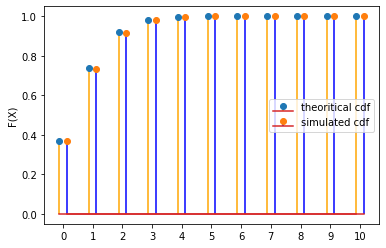
\includegraphics[width=\columnwidth]{solutions/xe/2019/simulated_theoritical.png}
    \caption{Theoretical CDF vs Simulated CDF}
    \label{Figure_0}
\end{figure}



\item \textbf{Step 1.} Flip a coin twice.\\
\textbf{Step 2.} If the outcomes are (TAILS, HEADS) then output Y and stop.\\
\textbf{Step 3.} If the outcomes are either (HEADS, HEADS) or (HEADS, TAILS), then output N and stop.\\
\textbf{Step 4.} If the outcomes are (TAILS, TAILS), then go to Step 1.\\
The probability that the output of the experiment is Y is (upto two decimal places)......
\\
%
\solution
Let flipping a coin twice be event H.\\
Sample space of event H = \cbrak{HH,HT,TH,TT}\\
Let a random variable X; $X_{i}=i$, where i=1,2,3. \\
 $X_{1}$ represents outcome \cbrak{TT}, 
 \\$X_{2}$ represents getting outcome \cbrak{TH} or output Y,
 \\ $X_{3}$ represents getting output N.\\
The state transition matrix P is shown below :
\begin{align}
\begin{array}{c c} &
\begin{array}{c c c} X_{1}  & X_{2} & X_{3} \\
\end{array}
\\
\begin{array}{c c c}
X_{1} \\
X_{2}\\
X_{3}
\end{array}
&
\left[
\begin{array}{c c c}
\frac{1}{4} & \frac{1}{4} & \frac{1}{2} \\
0 & 1 & 0 \\
0 & 0 & 1 
\end{array}
\right]
\end{array}
\end{align}
\\
\begin{figure}[h]
\caption*{\textbf{Markov chain diagram}}
\centering
\begin{tikzpicture}
       
             % Setup the style for the states
        \tikzset{node style/.style={state, 
                                    minimum width=1cm,
                                    line width=0.7mm,
                                    fill=gray!20!white}}
        % Draw the states
        \node[node style] at (3, 0)      (bull)     {$X_{1}$};
        \node[node style] at (0, -3)      (bear)     {$X_{2}$};
        \node[node style] at (6, -3) (stagnant) {$X_{3}$};
        % Connect the states with arrows
        \draw[every loop,
              auto=right,
              line width=0.7mm,
              >=latex,
              draw=orange,
              fill=orange]
           (bull)     edge[bend left=20]            node {$\frac{1}{2}$} (stagnant)
            (bull)     edge[bend right=20] node {$\frac{1}{4}$} (bear)
            
            
            (bull) edge[loop above]             node  {$\frac{1}{4}$} (bull)
            (bear) edge[loop below]             node  {1} (bear)
            (stagnant) edge[loop below]             node  {1} (stagnant);
    \end{tikzpicture}
\end{figure}\\
From the transition matrix, we have 1 transient state and 2 absorbing states.\\ Q = $\begin{bmatrix} \frac{1}{4} \end{bmatrix}$ and R = $\begin{bmatrix} \frac{1}{4} & \frac{1}{2} \end{bmatrix}$
\begin{align}
 N ={}& \brak{I - Q}^{-1}\\
 ={}& \brak{\sbrak{1} - \sbrak{\frac{1}{4}}}^{-1}\\
 ={}& \sbrak{\frac{4}{3}}
\end{align}
We know that probability of being absorbed by state j after starting in state i is given by the $M_{i,j}$, where M = NR.\\
\begin{align}
M = \begin{bmatrix} \frac{1}{3} & \frac{2}{3} \end{bmatrix}
\end{align}.\\
 Hence the probability of being absorbed by state Y $\brak{1^{st} \text{element of R}}$ after starting with state $X_{1}\brak{1^{st}\text{element of Q}}$ is $M_{1,1}$\\
 \\
\begin{align}
\therefore \pr{Y}=\frac{1}{3}=0.33 \brak{\text{correct upto 2 decimal places}}.
\end{align}

%
\item A fair coin is tossed till a head appears for the first time. The probability that the number of requried tosses is odd,is
\begin{enumerate}
\begin{multicols}{4}
\setlength\itemsep{2em}
\item $
\dfrac{1}{3}
$
\item $
\dfrac{1}{2}
$
\item $
\dfrac{2}{3}
$
\item $
\dfrac{3}{4}
$
\end{multicols}
\end{enumerate}
\solution
We can see that if the first toss is guaranteed to be a head, then the problem is reduced to finding the probability of getting one head in 2 coin tosses, since all the 3 trials are independent.
Let $K=\{0, 1, 2\}$ be the random variable denoting the number of heads obtained in 2 tosses of a fair coin. The event can be represented by a binomial distribution b(n,p).
In binomial distribution b(n,p), 
\begin{align}
Pr\brak{K=i}= \binom{n}{i}p^i \cdot (1-p)^{n-i}.
\end{align}
Here $n=2, p=0.5$.
 We can see that the probability of $K=1$ is 
 \begin{align}
 Pr\brak{K=1}&=\binom{2}{1} \cdot 0.5^2\\
 &=\frac{1}{2}
 \end{align}
 
From $\brak{2.0.1}$ and $\brak{2.0.2}$, we see that probability of getting exactly 2 heads in 3 tosses, if the first toss is a head, is 0.5.

%
\item Players A and B take turns to throw a fair dice with six faces. If A is the first player to throw, then the probability of B being the first one to get a six is --- ( round of to two decimal places). \\
\solution

Let the random variable X represent which player gets six first. That is $X=0 $ when A gets a six first and $X=1 $ when B gets six first. \\
Let another random variable Y represent getting a six on the dice. $Y=1 $ for six and $Y=0 $ for any other number. \\
Let N be the number of turns until we get a six.
\begin{align}
    \Pr\brak{Y=0} = \frac{5}{6} \\
    \Pr\brak{Y=1} = \frac{1}{6}
\end{align}
The event success is when B gets a six for first time and failure is when neither A nor B gets six. Let p denote probability of success 
\begin{align}
    p &= \Pr\brak{Y=1}  \\
    \Pr\brak{Y=0} &= 1- p \\
    p &= \frac{1}{6}
\end{align}
To get $X=1 $ in $N$ turns we have to get $N-1$ failures for B and $ N$ failures for A and finally one success for B. 
Therefore the geometric distribution is,
\begin{align}
    f(N) &= \brak{1-p}^{n-1} \times p \times  \brak{1-p}^{n} \\
    &  = \brak{1-p}^{2n-1} \times p \\
    & = \brak{ \frac{5}{6}}^{2n-1} \times \frac{1}{6}
\end{align}
The result has been summarized in table \ref{tab:table geometric distribution}. \\
\begin{table}[hbt!]
\centering
\begin{tabular}{|c|c|}
\hline
\textbf{No. of turns} & \textbf{Probability} \\ \hline
1                     & $5^1/6^2  $            \\ \hline
2                     & $5^3/6^4 $             \\ \hline
$\vdots  $              & $\vdots $              \\
n                     & $5^{2n-1}/6^{2n} $         \\ \hline
$\vdots $               & $\vdots $              \\ \hline
\end{tabular}
\caption{Summary of turns}
\label{tab:table geometric distribution}
\end{table}
Thus the total probability is sum of these individual probabilities i.e.
\begin{align}
    \Pr\brak{X=1} &= \sum_{N=1}^{\infty} f(N) \\
    &= \frac{5}{6^2} + \frac{5^3}{6^4} + \hdots + \frac{5^{2n-1}}{6^{2n}} +\hdots  \\
    &= \frac{5}{6^2} \times \brak{1 + \frac{5^2}{6^2} + \frac{5^4}{6^4} + \hdots } 
\end{align}
By Using sum of infinite GP we have, 
\begin{align}
     \Pr\brak{X=1} &= \frac{5}{6^2} \times \brak{\frac{1}{1 - \frac{25}{36}}}  \\
       &= \frac{5}{36} \times \frac{36}{11} \\
       &= \frac{5}{11} = 0.45
\end{align}


\end{enumerate}